% =====================================================================
% Small-Scale Text Diffusion for a Psychology Assistant
% arXiv preprint — audited write-up of the psyche_diffuse_60m project
% Build: pdflatex preprint.tex  (run twice for cross-references)
% Plain pdfLaTeX, no external figures, no .bib file required.
% Every number re-verified against on-disk artifacts on 2026-06-10;
% the claim->artifact audit map is Appendix A. Paths are repo-relative.
% =====================================================================
\documentclass[11pt]{article}

\usepackage[margin=1in]{geometry}
\usepackage{amsmath,amssymb}
\usepackage{booktabs}
\usepackage{array}
\usepackage{graphicx}
\usepackage{microtype}
\usepackage{xcolor}
\usepackage[colorlinks=true,linkcolor=blue!45!black,citecolor=blue!45!black,urlcolor=blue!45!black]{hyperref}
\usepackage{xurl}
\usepackage{caption}
\usepackage[numbers]{natbib}
\captionsetup{font=small,labelfont=bf}

\newcommand{\MASK}{\texttt{[MASK]}}
\newcommand{\repo}[1]{\texttt{\footnotesize #1}}
\newcommand{\sixsix}{66.8M}
\newcommand{\onetwenty}{120M}
\newcommand{\good}{\textcolor{green!45!black}{verified}}
\newcommand{\fixed}{\textcolor{orange!75!black}{corrected}}

\title{\bfseries Small-Scale Text Diffusion for a Psychology Assistant:\\
A Discrete-Diffusion Pipeline, a Blind-Annotation Retraction,\\
and an Honest Data-Bound Scaling Null}

\author{Denis Kim\\
\small Independent researcher\\
\small \texttt{kdleonidovich04@gmail.com}}

\date{June 2026\\[2pt]\small Working preprint. Single-GPU (RTX 3090) study; all artifacts in the project repository.}

\begin{document}
\maketitle

\begin{abstract}
We build an English psychology / mental-health text-generation model on a single consumer GPU and report the full chain of results --- several of them negative --- with deliberate measurement rigor. The methodological spine is a self-caught error: an effect we first ``found'' non-blind (corpus cleaning halving confabulation, $57\%\!\to\!29\%$) \emph{vanished under blind annotation} (Fisher $p=1.0$); we retract it and treat the caught confirmation bias, and the blind protocol that exposed it, as a primary contribution. Substantive findings: (1)~\textbf{Architecture} --- continuous (Gaussian) text diffusion at 60.8M parameters / 2.56B tokens produces topic-coherent \emph{word salad}, while discrete masked diffusion (MDLM) on the same data, tokenizer, and token budget --- at a marginally \emph{larger} 66.8M, a gap the scale-axis null (\S\ref{sec:scale}) shows is immaterial --- yields grammatical sentences. (2)~\textbf{Decoding} --- the discrete model's dominant failure, repetition collapse, is a \emph{decode artifact, not a capacity limit}: confidence-based unmasking plus repetition controls remove it with no weight change (rep-1 $-53\%$ at fixed temperature). (3)~\textbf{Data} --- a strict-filtered 0.77B-token corpus is $3.3\times$ cheaper than the 2.56B noisy corpus and no worse on the most sensitive eval (paired cosine $d=+0.0094$, win-rate $0.527$): cleaning buys \emph{cost}, not quality. (4)~\textbf{Scale} --- doubling to 120M parameters at fixed data moves neither aggregate quality (paired $d=-0.0094$, win-rate $0.479$) nor the blind homonym-drift floor (Fisher $p=0.77$); a measured null we attribute to an \emph{inferred} data-bound regime (6.4 vs.\ 11.6 tokens/param against a $\approx$20 optimum), falsifiable only by a data-fed rerun. The shipped model is the cheaper \sixsix\ clean checkpoint, deployed fully on-device (Android, ONNX, fp32). A closing audit re-derived every headline statistic from raw artifacts (Appendix~\ref{app:audit}).
\end{abstract}

\paragraph{Intended use, limitations, and safety.} This is a research artifact for studying small-scale text diffusion, \emph{not} a clinical, diagnostic, or psychological tool. The model was validated on no clinical endpoint, carries no regulatory clearance, and its outputs are frequently vague, repetitive, and factually wrong --- a blind homonym-drift floor of 25--32\% persists at both model sizes (\S\ref{sec:scale}). It must not be used for diagnosis, treatment, or crisis support, and the on-device demo (\S\ref{sec:deploy}) is an engineering proof-of-concept, not a product. For crisis support contact 988 (US) or a local emergency line. The training data contain no real conversations and no personally identifying information.

\paragraph{Code, model, and artifacts.} Code, evaluation artifacts (blind keys, annotator labels, eval harness), and the \LaTeX\ source of this paper: \url{https://github.com/thunder-phoenix-lab/research-psyche-diffuse-66m}. Model weights (66.8M production checkpoint + 120M scale checkpoint, SentencePiece tokenizer, ONNX mobile export): \url{https://huggingface.co/tp-di/psyche-diffuse-66m}. Every headline number recomputes bit-exactly from the shipped artifacts (Appendix~\ref{app:audit}).

% =====================================================================
\section{Introduction}
% =====================================================================

The goal was a compact diffusion language model specialized to psychology and mental-health dialogue, trainable and deployable on one RTX~3090. Diffusion LMs promise controllable, non-autoregressive generation, but little is documented about what works at the small scale a hobbyist or edge budget allows. This paper is an engineering-and-science log: what failed, what worked, and where our own measurements misled us until corrected.

The project ran as seven stages. For each, the body states \emph{what was done}, \emph{why}, and \emph{what it led to} --- the causal chain matters, because three pivots (architecture switch, sampler rewrite, corpus rebuild) were each forced by a documented negative result, and one headline ``positive'' was retracted on its own evidence:

\begin{enumerate}\itemsep1pt
\item \textbf{Data + tokenizer} (\S\ref{sec:setup}): 2.56B-token psychology-dominant corpus, 261k-pair SFT set, fixed 16k SentencePiece vocab $\rightarrow$ one tokenizer and recipe frozen for every later arm.
\item \textbf{Continuous diffusion, v1--v3} (\S\ref{sec:cont}): topic control emerged; grammar never did; five extra sampler tricks made outputs strictly worse $\rightarrow$ pivot to discrete diffusion at identical budget.
\item \textbf{Discrete MDLM} (\S\ref{sec:mdlm}): same scale, grammatical English $\rightarrow$ pipeline gate opened.
\item \textbf{Decode fix} (\S\ref{sec:decode}): repetition collapse removed with zero retraining $\rightarrow$ collapse $=$ decode order, sampler frozen for all evals and deployment.
\item \textbf{Clean corpus + factorial} (\S\ref{sec:clean}--\ref{sec:retraction}): strict filter to 0.774B tokens; non-blind ``confab halved'' \emph{retracted} under blind labels $\rightarrow$ standing blind protocol.
\item \textbf{Data and scale axes} (\S\ref{sec:data}--\ref{sec:scale}): paired 1000-prompt eval + blind traps $\rightarrow$ cleaning buys cost not quality; $2\times$ params at fixed data is a null.
\item \textbf{Deployment} (\S\ref{sec:deploy}): \sixsix-clean exported to ONNX, runs on-device.
\end{enumerate}

\textbf{Related work.} The discrete model follows masked-diffusion LMs --- MDLM \citep{sahoo2024mdlm}, SEDD \citep{lou2024sedd} --- with confidence-ordered unmasking from MaskGIT \citep{chang2022maskgit}; the continuous baseline is Diffusion-LM \citep{li2022diffusionlm} with DiffuSeq-style conditioned SFT \citep{gong2023diffuseq}; the backbone is a DiT \citep{peebles2023dit}. Scaling is read through Chinchilla \citep{hoffmann2022chinchilla}; the data result confirms, in the diffusion regime, the curated-small-data line of TinyStories \citep{eldan2023tinystories} and phi \citep{gunasekar2023textbooks}. The combination --- masked diffusion, single GPU, domain-specialized, with a blind-annotation retraction --- is, to our knowledge, not covered by these.

% =====================================================================
\section{Setup: model, objective, data}\label{sec:setup}
% =====================================================================

\paragraph{Backbone.} Diffusion Transformer with AdaLN-zero timestep conditioning, RMSNorm, SwiGLU MLP, SDPA attention, learned positions, tied output head ($\mathrm{logits}=hE^{\top}+b$), sequence length 512. Two sizes (Table~\ref{tab:arch}); \onetwenty\ scales width and depth at fixed head dim 64. Training is pure bf16 --- parameters, activations, gradients; fp32 only inside RMSNorm, the sinusoidal time embedding, and loss reductions --- with AdamW8bit \citep{dettmers2022adamw8bit}, no fp32 master weights. This single-card regime is held constant across all arms, so it is not a confound for any comparison.

\begin{table}[h]\centering\small
\caption{Architectures. Parameter counts are from training-log prints, not estimates.}
\label{tab:arch}
\begin{tabular}{lcccccc}
\toprule
name & hidden & layers & heads & MLP inter & params & tok/param @0.774B \\
\midrule
\sixsix    & 512 & 12 & 8  & 1408 & 66.8M  & 11.6 \\
\onetwenty & 640 & 15 & 10 & 1664 & 121.4M & 6.4 \\
\bottomrule
\end{tabular}
\end{table}

\paragraph{Objective.} MDLM \citep{sahoo2024mdlm}: per sequence draw $t\sim U(0.01,0.99)$, mask each token independently with probability $t$ (vocab $16{,}000+1$ \MASK), cross-entropy on masked positions only. SFT is DiffuSeq-style: only response positions are noised, prompts stay clean as conditioning; zero new parameters, pretrain checkpoint loaded \texttt{strict=True}.

\paragraph{Recipe (frozen).} Batch 32 $\times$ accum 8 ($=256$ seqs $=131$k tokens/step), LR $4{\cdot}10^{-4}$ cosine, 2\% warmup, weight decay 0.1, betas $(0.9,0.99)$, clip 1.0; pretrain 20k steps ($\approx$2.62B seen tokens $=\,\approx$1 epoch noisy / $\approx$3.4 epochs clean), SFT 8k. Wall-clock per run on the 3090: $\approx$9.3h pretrain + 3.7--3.85h SFT at \sixsix; $\approx$26.5h + 5.8h at \onetwenty\ (run ledger: Appendix~\ref{app:runs}).

\paragraph{Data.} Pretrain corpus, psychology-dominant English, two versions: \textbf{noisy} 2{,}559{,}832{,}146 tokens / 2{,}163{,}570 docs ($\approx$69\% loosely psych-filtered Pile, plus peS2o, OpenAlex psychology, PMC, Gutenberg, PsyArXiv, and a small RU$\to$EN translated set); \textbf{clean} 773{,}925{,}936 tokens / 832{,}822 docs (\S\ref{sec:clean}). SFT: 261{,}443 (prompt,\,response) pairs at length 512 (assistant + mental-health + translated psychology dialogue), shared by every arm. We do \emph{not} redistribute the corpora --- the noisy mix is $\approx$69\% Pile-derived and the SFT mix has heterogeneous source licenses --- but release the exact filter/build scripts and token/doc counts so both versions are reconstructible; the 1000-question eval set ships as prompts, with gold answers rebuildable from the source datasets.

\paragraph{What it led to.} Every later contrast changes one factor on identical infrastructure. The one violation of this rule was the non-blind labeling episode (\S\ref{sec:retraction}) --- caught and retracted.

% =====================================================================
\section{Stage 1 --- continuous diffusion fails, three samplers deep}\label{sec:cont}
% =====================================================================

We first built a continuous, $x_0$-parameterized Diffusion-LM-style model: 60.8M params, 2.56B tokens, DDIM, classifier-free guidance, self-conditioning.

\textbf{v1--v2.} CFG controls topic: at cfg${\approx}2.5$ outputs lock into a therapy register (on-topic content-word density ${\sim}10\%\!\to\!{\sim}35\%$), and constraints/clamp suppress garbage. Grammar never emerges --- outputs are word salad in the right vocabulary; CBT-vs-ACT and Vygotsky prompts fail outright. \textbf{v3 (negative).} Five further techniques (CFG cosine ramp, stochastic DDIM, final top-$p$/temp, iterative refinement, short max-length) were ablated on the same checkpoint: together they made outputs strictly worse --- register lock-in 3/5$\to$0/5, on-topic density ${\sim}35\%\!\to\!{\sim}15\%$; final top-$p$ over 16k SPM occasionally emits rare-Unicode one-shots.

\textbf{What it led to.} Inference-time engineering has a ceiling and we hit it: the limit is architectural. The arm survives only as a matched-budget baseline.

% =====================================================================
\section{Stage 2 --- discrete MDLM gives grammar at the same scale}\label{sec:mdlm}
% =====================================================================

The \sixsix\ pretrain reached masked-CE $9.80\!\to\!4.28$ (token acc 29.9\%) in 20k steps; SFT $4.80\!\to\!3.71$ (35.8\%). Coherent clauses appeared at 20\% of training; post-SFT, coping/advice prompts produce grammatical multi-sentence on-topic English --- the failure mode shifted to repetition collapse on factual/homonym prompts, expected at 60M.

\textbf{What it led to.} The architecture finding (discrete $\gg$ continuous at small scale, holding scale/data/tokenizer fixed), a frozen pipeline for matched experiments, and a defined next target: collapse.

% =====================================================================
\section{Stage 3 --- repetition collapse is decode-bound}\label{sec:decode}
% =====================================================================

Replacing random-order unmasking with confidence-ordered unmasking (cosine schedule) plus repetition penalty 1.3, neighbor-ban 2, no-repeat-3-gram fixes the same checkpoint, no retraining (Table~\ref{tab:decode}).

\begin{table}[h]\centering\small
\caption{v1 vs.\ v2 sampler, identical \sixsix-noisy weights, 5 matched prompts, temp fixed 0.9.}
\label{tab:decode}
\begin{tabular}{lccc}
\toprule
metric & v1 random & v2 conf+rep & $\Delta$ \\
\midrule
distinct-1 & 0.647 & 0.835 & $+29\%$ \\
distinct-2 & 0.929 & 0.971 & $+0.042$ \\
rep-1 & 0.353 & 0.165 & $-53\%$ \\
max-token-freq & 0.090 & 0.064 & $-29\%$ \\
\bottomrule
\end{tabular}
\end{table}

A first draft compared v1 at temp $\{0.7,1.0\}$ to v2 at $0.9$ and showed rep-1 $-62\%$; rerun at fixed 0.9 the effect attenuated to $-53\%$ --- part of the original delta \emph{was} temperature, and the controlled number is reported. \textbf{What it led to:} collapse $=$ decode order, not capacity; sampler frozen for all evals (and the phone). The decode fix did \emph{not} reduce homonym drift, isolating it as a data/capacity question.

% =====================================================================
\section{Stage 4 --- strict-filtered clean corpus}\label{sec:clean}
% =====================================================================

Drift such as \emph{Vygotsky}$\to$``coastal/coral'' implicated the Pile component. Strict filter --- keep iff core-psych hits $\ge3$ and core $\ge$ off-domain --- yields 0.774B tokens (30\% of noisy) at far higher purity; the standing rule --- \emph{``never weaken the filter to buy tokens''} --- held, accepting under-feeding of \onetwenty. A pretrain-level probe (clean stays developmental on \emph{proximal/distal}; noisy drifts to islands) motivated --- but does not establish --- a corpus effect; that test is \S\ref{sec:retraction}. \textbf{Led to:} the corpus axis and the $3.3\times$ cheaper production model.

% =====================================================================
\section{Stage 5 --- the retracted finding and the blind protocol}\label{sec:retraction}
% =====================================================================

Factorial: decode (v1/v2) $\times$ corpus (noisy/clean) at \sixsix. Decode reproduced on both corpora. On 14 homonym traps $\times$ 2 seeds the author labeled drift \emph{knowing condition and hypothesis}: $16/28$ vs $8/28$ --- ``cleaning halves confabulation''. Three checks before publishing:
(1)~\textbf{CIs}: Wilson $[0.39,0.73]$ vs $[0.15,0.47]$, Fisher $p=0.058$ --- not significant.
(2)~\textbf{Blind} (decisive): 56 pooled, shuffled, source-stripped items, labeled by two fresh, independent annotators --- LLM (Claude) sub-agents with no memory of the project and no exposure to source, hypothesis, or condition (verbatim task spec in Appendix~\ref{app:prompts}). Using fresh LLM sub-agents rather than the author is what makes the blind protocol cheap enough to run as standing practice:

\begin{center}\small
\begin{tabular}{lccc}
\toprule
annotator & noisy & clean & Fisher $p$ \\
\midrule
author, non-blind & 16/28 (57\%) & 8/28 (29\%) & 0.058 \\
A, blind & 11/28 (39\%) & 10/28 (36\%) & 1.000 \\
B, blind & 7/28 (25\%) & 7/28 (25\%) & 1.000 \\
\bottomrule
\end{tabular}
\end{center}

$\kappa_{AB}=0.71$: criterion reliable, effect absent --- the non-blind delta was confirmation bias.
(3)~\textbf{Specificity}: clean is not blander (TTR $0.899$ vs $0.900$; content-word $0.556$ vs $0.562$; hapax $0.910$ vs $0.907$).

\textbf{Retraction; reading.} Trap drift splits ${\sim}14/16$ homonym-type (\emph{drive}$\to$vehicles) --- corpus-invariant lexical floor --- vs ${\sim}2/16$ contamination-type, all cleaning can fix. \textbf{Led to:} standing protocol --- pool, shuffle, strip, $\ge$2 fresh blind annotators, decode after, report $\kappa$/CI/Fisher --- used throughout \S\ref{sec:scale}.

% =====================================================================
\section{Stage 6a --- data axis: cleaning buys cost, not quality}\label{sec:data}
% =====================================================================

Same arch/SFT; pretrain clean 0.774B vs noisy 2.56B. Ceiling metrics: tie (above). Degeneration, 1000 prompts: distinct-2 0.993/0.991, rep-1 0.137/0.141, zero collapse. Sensitive eval, MiniLM cosine-to-gold on 725 paired prompts: 0.500 vs 0.490, $d=+0.0094$, CI $[+0.0003,+0.0186]$, $t(724)=2.01$, win 0.527 --- borderline significant, negligible size. \textbf{Led to:} cleaning's benefit is cost ($3.3\times$ fewer tokens, no penalty); confirms TinyStories/phi in diffusion. Caveats: volume/purity confounded (noisy-0.77B not run); slim fluency edge $\neq$ trap result (\S\ref{sec:retraction}); the $\pm0.0094$ symmetry with \S\ref{sec:scale} is coincidental (not engineered or tuned) --- it shows the metric resolves 0.01, but the signs are single-seed.

% =====================================================================
\section{Stage 6b --- scale axis: a data-bound null}\label{sec:scale}
% =====================================================================

\onetwenty\ on identical clean data (transient CUDA fault absorbed by auto-resume). Pre-registered evals:
\textbf{Aggregate paired:} 0.490 vs 0.500, $d=-0.0094$, CI $[-0.0188,-0.0001]$, $t=-1.96$, win 0.479 --- practical tie. \textbf{Blind traps} (3 fresh blind annotators --- again independent Claude sub-agents, \S\ref{app:prompts} --- $\kappa$ 0.767/0.867/0.825): \onetwenty\ 7/28 vs \sixsix\ 9/28, Newcombe $[-0.294,+0.161]$, Fisher $p=0.768$ --- floor 25--32\% both. \textbf{Led to:} measured null; inferred data-bound mechanism (6.4 vs 11.6 tok/param, optimum ${\approx}20$); production $=$ \sixsix-clean. Scope: single seed/cell, two checkpoints, in-distribution golds; falsifier $=$ 2.4B-token \onetwenty.

% =====================================================================
\section{Stage 7 --- on-device deployment; conclusions}\label{sec:deploy}
% =====================================================================

\sixsix-clean exported to ONNX ($286$~MiB $=300$~MB asset; debug APK 365~MB), ONNX Runtime Mobile CPU, fp32 inference of bf16 weights (no quantization), v2 sampler ported, diffusion visualized (Figure~\ref{fig:app}).

\textbf{Limitations.} Every contrast is a single seed and a single checkpoint per cell on one GPU; we report paired tests and confidence intervals but no across-seed variance, so the small effects (\S\ref{sec:data}--\ref{sec:scale}) should be read as point estimates, not population claims. Evaluation golds are in-distribution to the SFT sources, the scale null is at one (under-fed) data budget, and all blind labels come from LLM (Claude) sub-agents rather than human clinicians --- internally consistent ($\kappa$ .71--.87) but not a substitute for expert human annotation. These are the obvious targets for a follow-up.

\textbf{Conclusions:} discrete $>$ continuous at small scale; collapse is a decode problem; cleaning buys cost, not quality; doubling params at fixed data buys nothing measured; and \emph{blind annotation --- here cheap because the annotators are fresh LLM sub-agents --- is non-negotiable}: it is what turned our own headline ``positive'' into a retraction.

\begin{figure}[h]\centering

\includegraphics[width=0.295\textwidth]{figs/screenshot_v2_crop.png}\hspace{0.04\textwidth}
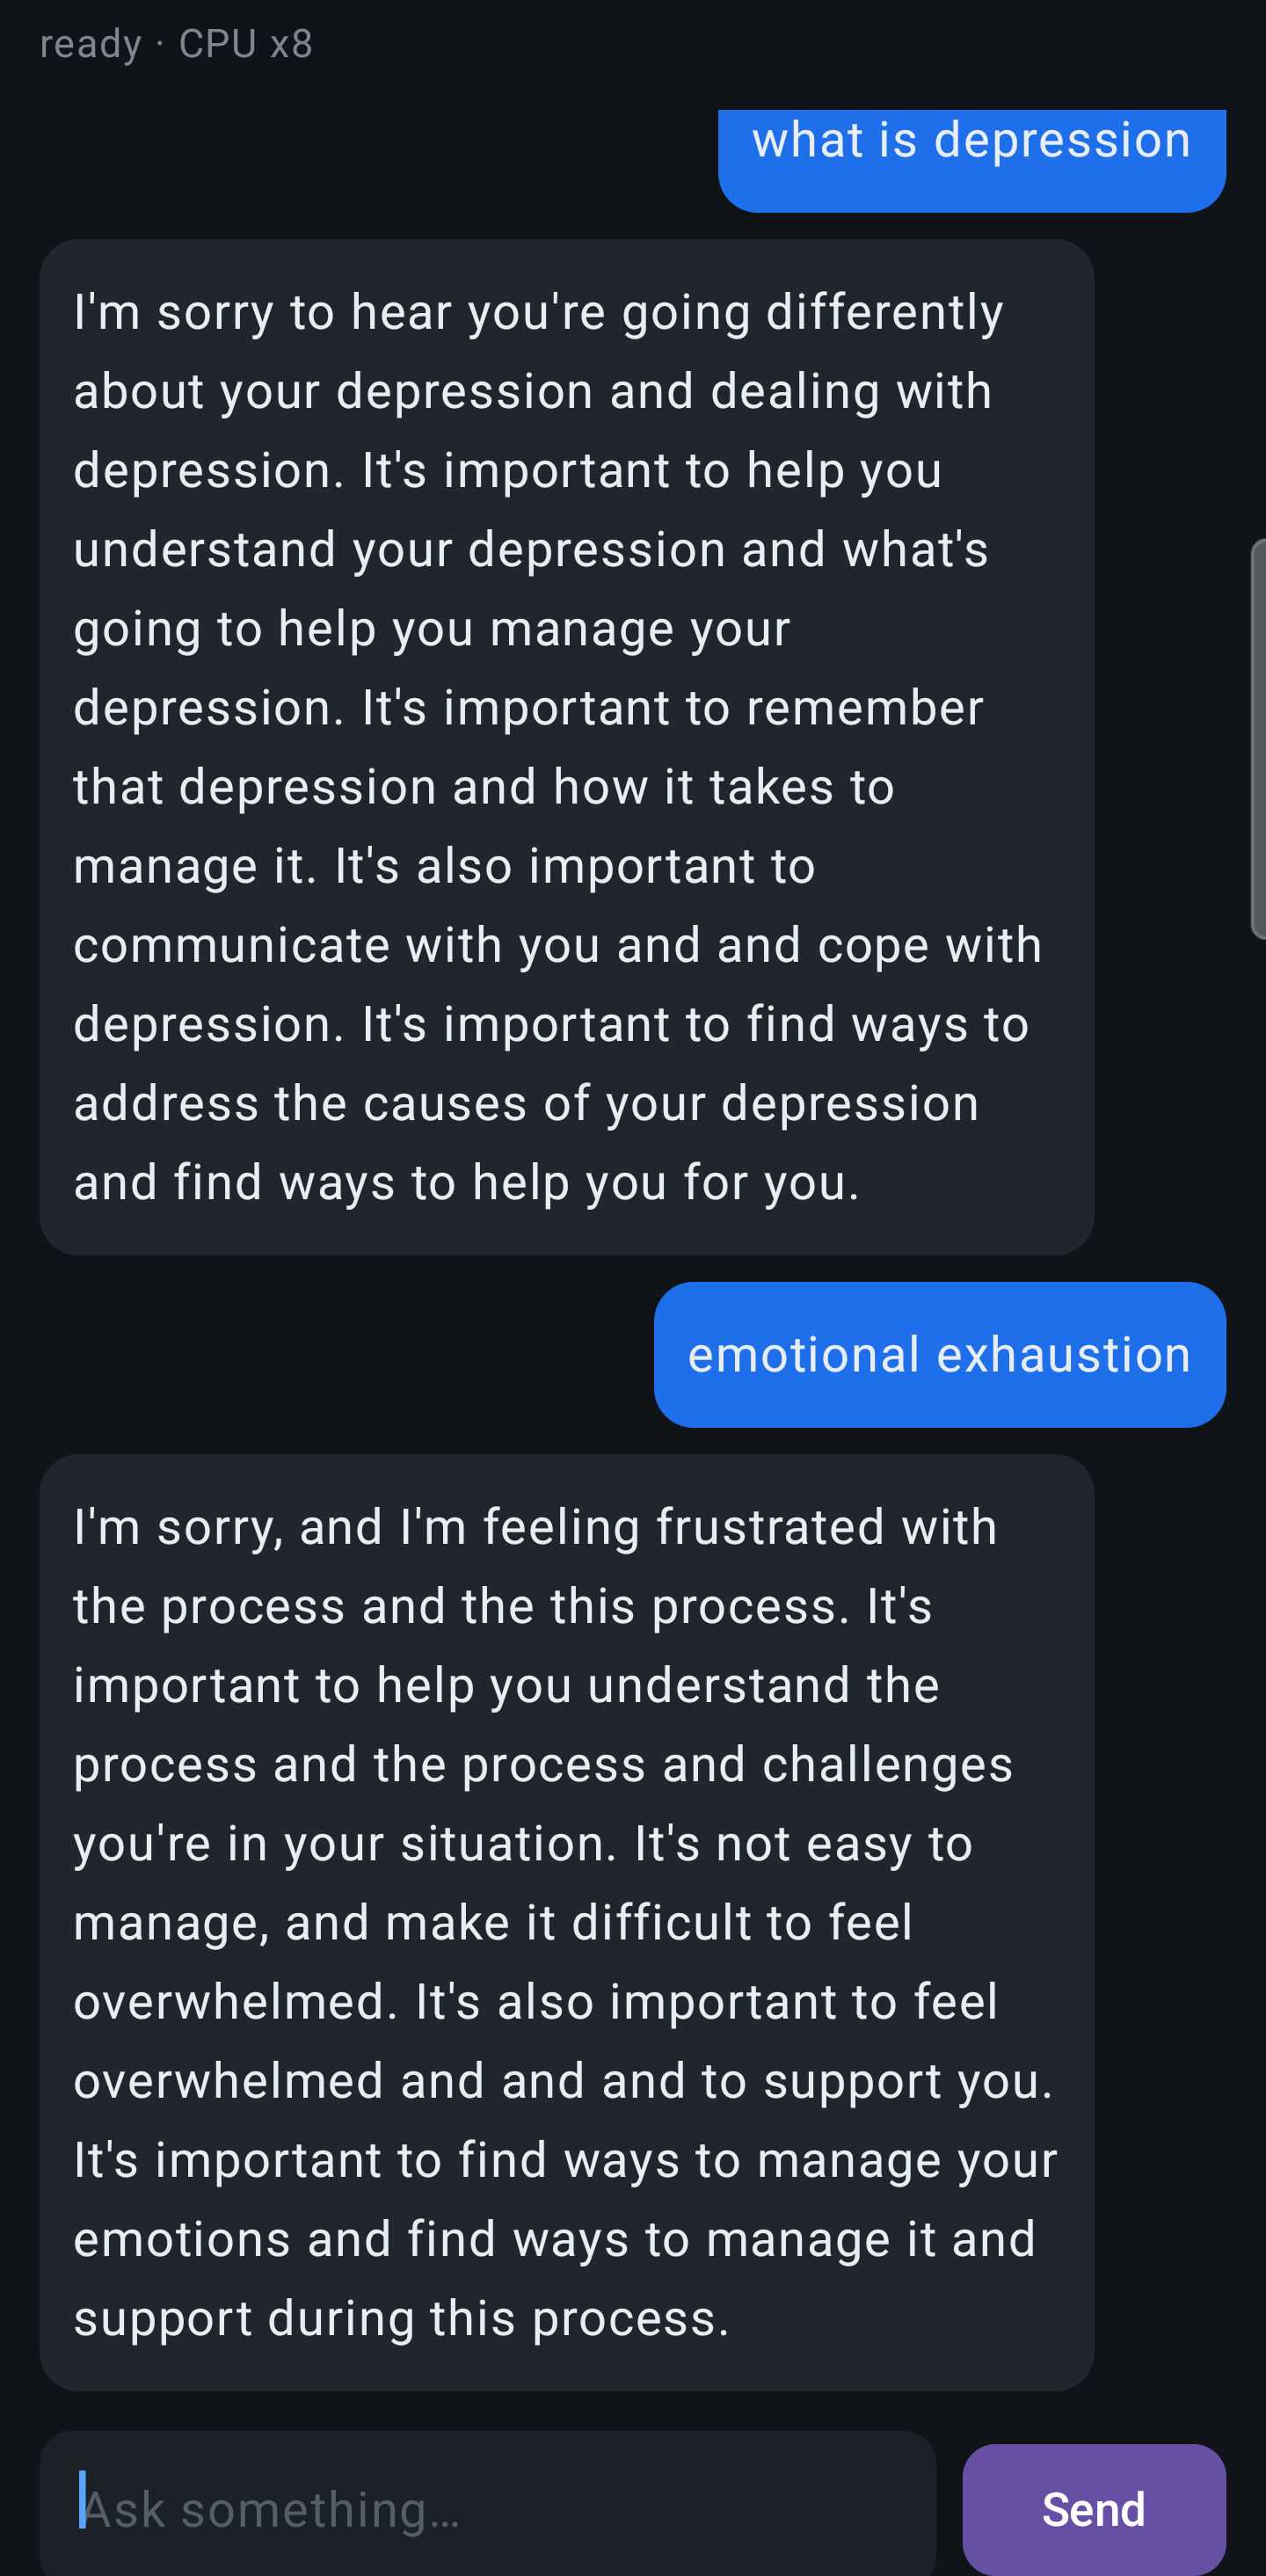
\includegraphics[width=0.295\textwidth]{figs/screenshot_v3_crop.png}
\caption{The \sixsix-clean model on a phone (ONNX Runtime Mobile, 8 CPU threads). The two panels are different settings, not a before/after of the same run. Left: masked-diffusion decoding mid-generation under an 18-step preview schedule (step 4/18) --- unmasked tokens appear in confidence order. Right: completed chat answers under the frozen evaluation/production \S\ref{sec:decode} sampler (28 steps, temp 0.9, rep 1.3). Outputs are grammatical, on-topic, mildly repetitive --- consistent with the limitations stated for this scale.}
\label{fig:app}
\end{figure}

\appendix
% =====================================================================
\section{Audit map: every headline number, claim $\to$ artifact $\to$ status}\label{app:audit}
% =====================================================================

A closing audit (2026-06-10) re-derived each headline statistic from raw on-disk artifacts rather than from the working notes. Counts were verified against \repo{meta.json} and byte sizes; the blind-trap statistics were recomputed by rerunning \repo{eval/score\_blind\_traps.py} over the archived key and annotator files; the paired cosines were recomputed end-to-end (re-embedding all outputs) with \repo{eval/paired\_sig.py}.

\begin{table}[h]\centering\footnotesize
\caption{Claim $\to$ artifact $\to$ recomputed value. Paths relative to \repo{raw\_data/004\_train/}.}
\begin{tabular}{>{\raggedright\arraybackslash}p{0.30\textwidth}>{\raggedright\arraybackslash}p{0.30\textwidth}>{\raggedright\arraybackslash}p{0.30\textwidth}}
\toprule
claim & artifact & recomputed \\
\midrule
noisy corpus 2.56B tok, 2.16M docs & \repo{pretrain\_en\_diff\_clean/} \repo{meta.json} & 2{,}559{,}832{,}146; \good \\
clean corpus 0.774B tok, 833k docs & \repo{pretrain\_en\_clean\_v2/} \repo{meta.json} & 773{,}925{,}936; \good \\
SFT 261{,}443 pairs $\times$ 512 & \repo{sft\_en/meta.json}, bin size & exact; \good \\
params 66.8M / 121.4M & run logs & \good \\
runs 20k pre, 8k SFT, $\times 6$ & six \repo{mdlm\_*.log}, 05-29..31 & steps and dates \good \\
decode fix (Table~\ref{tab:decode}) & \repo{RESULTS\_matched...md} & \good\ (temp-controlled) \\
retraction $p$ values & 56-sample key, counts & 0.058 / 1.000 / 1.000; \good \\
data axis $d=+0.0094$ & 725 pairs re-embedded & $[+0.0003,+0.0186]$, $t{=}2.01$, win 0.527; \good \\
scale axis $d=-0.0094$ & 725 pairs re-embedded & $[-0.0188,-0.0001]$, $t{=}-1.96$, win 0.479; \good \\
blind scale traps & \repo{annot\_\{A,B,C\}.txt}, key & 7/28 vs 9/28, $p{=}0.768$, $\kappa$ .77/.87/.83; \good \\
1000-Q set, gold pairs & line counts & 1000, 725; \good \\
ONNX asset ``$\approx$243 MB'' & app assets dir & 286.4 MiB $=$ 300.3 MB; \fixed \\
\bottomrule
\end{tabular}
\end{table}

Archival notes: the \S\ref{sec:retraction} blind labels survive as counts in the results file (per-sample files were kept only for the scale round, which fully recomputes); the \emph{noisy} dataset lives in the historically named directory \repo{pretrain\_en\_diff\_clean} (the clean one is \repo{pretrain\_en\_clean\_v2}); Wilson upper bound for 16/28 rounds to 0.73 (notes printed 0.74).

% =====================================================================
\section{Blind annotation protocol (standing)}
% =====================================================================
(1)~Generate condition pools (here $2$ seeds $\times$ 14 traps per checkpoint). (2)~Pool, shuffle, strip identifiers; assign neutral IDs (\repo{build\_blind\_traps*.py}). (3)~$\ge$2 (latterly 3) fresh annotators --- LLM sub-agents never exposed to source, hypothesis, or direction --- label drift yes/no per item; criterion only. (4)~Decode by key; report per-source rates, Wilson 95\% CIs, Newcombe diff CI, two-sided Fisher exact, pairwise Cohen $\kappa$ (\repo{score\_blind\_traps.py}). (5)~A non-blind label may motivate, never headline. Triggered: the author 57\% vs 29\% became blind $p=1.0$.

% =====================================================================
\section{Verbatim prompts given to the LLM sub-agents (Claude)}\label{app:prompts}
% =====================================================================

All annotation and curation labor besides the author was performed by fresh Claude sub-agents (Claude Code \texttt{Agent} tool, general-purpose, one task per agent, no memory of the project, no access to hypotheses or checkpoint identities).

\paragraph{Blind drift annotators (\S\ref{sec:retraction}, \S\ref{sec:scale}).} Each annotator received only the pooled, shuffled, source-stripped sample file (\repo{blind\_traps*.txt}); its header is the entire task specification. Scale round, verbatim (the \S\ref{sec:retraction} round was identical except the domain list lacked physics/cosmology and economics):
\begin{quote}\small\ttfamily\raggedright
Label each item DRIFT=yes/no. DRIFT=yes if a substantial part of the response is about a NON-psychology domain (physics/cosmology, marine biology, automotive, military, pure statistics/math, programming, geometry, economics, anatomy-as-physiology, etc). DRIFT=no if it stays within psychology/therapy/cognition/development EVEN IF factually wrong, vague, or repetitive. Repetition or incoherence alone is NOT drift.
\end{quote}
Annotators returned one \texttt{Sxxx: yes/no} line per item (files \repo{annot\_A}--\repo{C.txt}); decoding against the key happened only afterwards.

\paragraph{1000-question curators (\S\ref{sec:data}--\ref{sec:scale}).} Candidate questions were machine-extracted in-distribution from the three SFT sources, psych-filtered, deduplicated, and split into 20 shards of 150; each of 20 sub-agents was instructed to curate, from its shard, the best 50 distinct well-formed English psychology questions, with a further 8 agents reconciling overlaps to exactly 1000; gold answers were recovered for 725 by matching SFT targets. Scripts: \repo{build\_q\_shards.py}, \repo{build\_eval\_pairs.py}. Curators never saw model outputs, so the prompt set predates and is independent of every model under comparison.

% =====================================================================
\section{Run ledger (verified from logs)}\label{app:runs}
% =====================================================================
\begin{center}\small
\begin{tabular}{llll}
\toprule
run & steps & wall & checkpoint \\
\midrule
mdlm\_v1 (noisy pre) & 20k & 05-29 00:47--10:05 & \repo{mdlm\_v1/final} \\
mdlm\_sft (noisy) & 8k & 10:06--13:48 & \repo{mdlm\_sft/final} \\
mdlm\_v1\_clean & 20k & 15:30--00:45 & \repo{mdlm\_v1\_clean/final} \\
mdlm\_sft\_clean (prod) & 8k & 00:49--04:38 & \repo{mdlm\_sft\_clean/final} \\
mdlm\_120m & 20k & 05-29--05-30 21:47 & \repo{mdlm\_120m/final} \\
mdlm\_sft\_120m & 8k & 21:50--03:39 & \repo{mdlm\_sft\_120m/final} \\
\bottomrule
\end{tabular}
\end{center}

\begin{thebibliography}{10}\small
\bibitem[Sahoo et al.(2024)]{sahoo2024mdlm} Sahoo, S. et al. Simple and Effective Masked Diffusion Language Models. NeurIPS 2024. arXiv:2406.07524.
\bibitem[Lou et al.(2024)]{lou2024sedd} Lou, A. et al. Discrete Diffusion Modeling by Estimating the Ratios of the Data Distribution (Score Entropy Discrete Diffusion). ICML 2024. arXiv:2310.16834.
\bibitem[Chang et al.(2022)]{chang2022maskgit} Chang, H. et al. MaskGIT: Masked Generative Image Transformer. CVPR 2022. arXiv:2202.04200.
\bibitem[Li et al.(2022)]{li2022diffusionlm} Li, X. et al. Diffusion-LM Improves Controllable Text Generation. NeurIPS 2022. arXiv:2205.14217.
\bibitem[Gong et al.(2023)]{gong2023diffuseq} Gong, S. et al. DiffuSeq: Sequence to Sequence Text Generation with Diffusion Models. ICLR 2023. arXiv:2210.08933.
\bibitem[Hoffmann et al.(2022)]{hoffmann2022chinchilla} Hoffmann, J. et al. Training Compute-Optimal Large Language Models. NeurIPS 2022. arXiv:2203.15556.
\bibitem[Eldan and Li(2023)]{eldan2023tinystories} Eldan, R. and Li, Y. TinyStories: How Small Can Language Models Be and Still Speak Coherent English? 2023. arXiv:2305.07759.
\bibitem[Gunasekar et al.(2023)]{gunasekar2023textbooks} Gunasekar, S. et al. Textbooks Are All You Need. 2023. arXiv:2306.11644.
\bibitem[Peebles and Xie(2023)]{peebles2023dit} Peebles, W. and Xie, S. Scalable Diffusion Models with Transformers. ICCV 2023. arXiv:2212.09748.
\bibitem[Dettmers et al.(2022)]{dettmers2022adamw8bit} Dettmers, T. et al. 8-bit Optimizers via Block-wise Quantization. ICLR 2022. arXiv:2110.02861.
\end{thebibliography}
\end{document}
